	\section{Получение и первичная обработка данных}
	
	
			\begin{wrapfigure}[17]{l}{0.6\linewidth}
\singlespacing
\vspace{-35px}
%  \begin{center}
    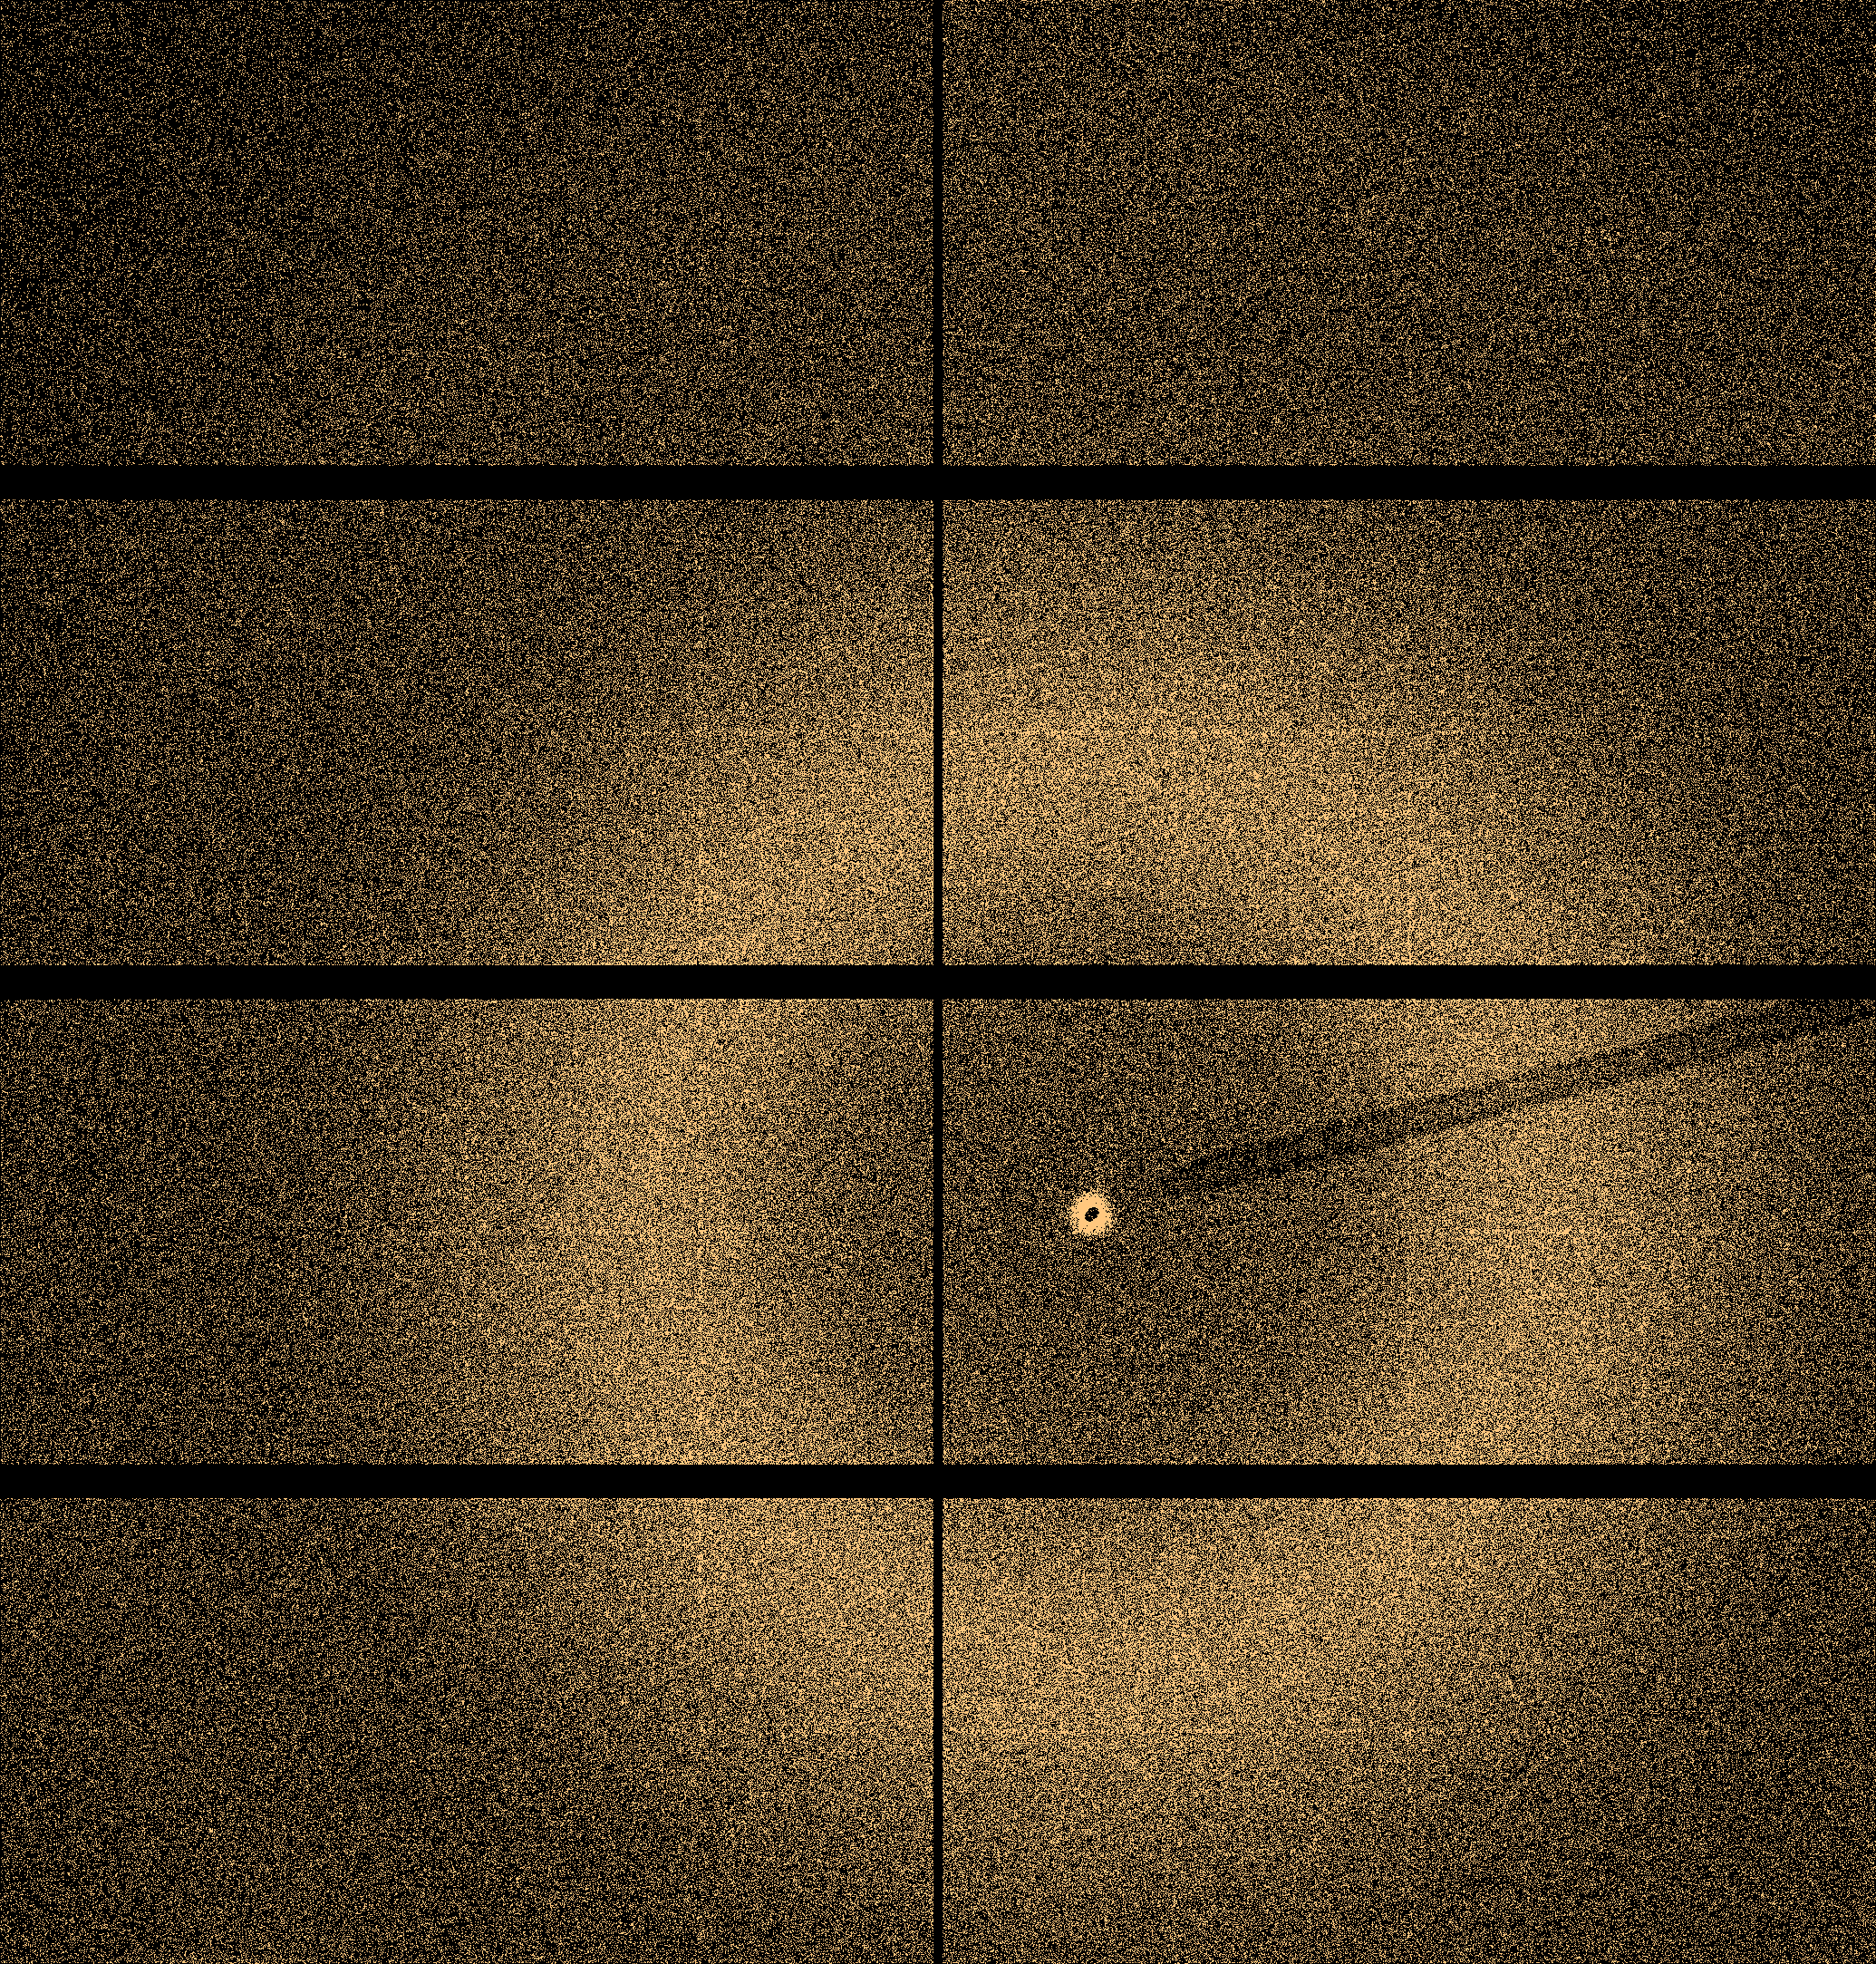
\includegraphics[width=0.9\linewidth]{fig/obj.png}
    \vspace{3px}
    \caption{Изображение с 2D~-детектора. Черные области соответствуют промежуткам между элементами детектора, затемненная облась справа  - тень от бимстопа}
    \label{fig:difractogram}
%  \end{center}
\end{wrapfigure}
	
	
	Детектирование картин дифракции при сканировании образца наноразмерным пучком рентгеновского синхротронного излучения производится с шагом 1 мкм вдоль образца. 
	Это позволяет установить, что образцы полиимидных порошков и пленок не являются однородным, а имеют как чисто аморфные, так и частично-кристаллические участки.
	Типичное изображение, получаемое на детекторе для единичного измерения, представлено на рис. \ref{fig:difractogram}. Различие в сигналах кристаллических и аморфных областей хорошо видно на фрагментах дифрактограмм, преобразованных к полярной системе координат, представленных на рис. \ref{fig:azim}. Как видно из рисунка, наличие кристаллической фазы приводит к появлению двух основных дифракционных пиков, в то время как рассеяние на чисто аморфных участках дает только так называемое аморфное гало.
	
		\begin{figure}[t]\center
\begin{tabular}{cc}
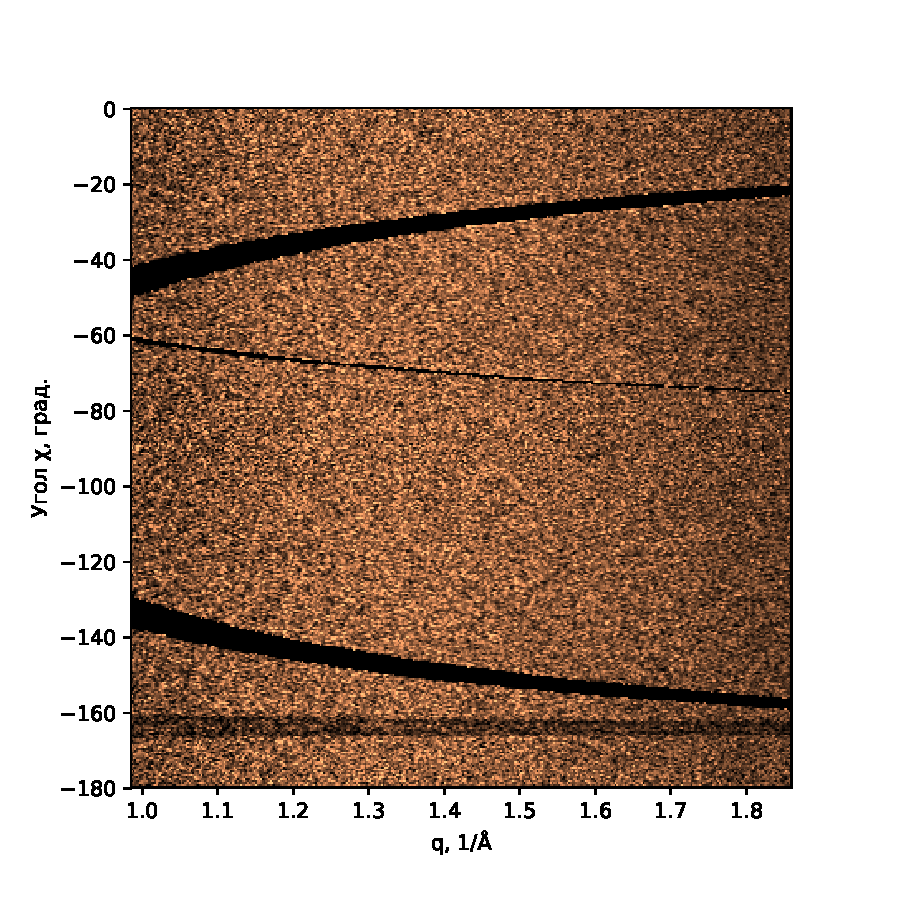
\includegraphics[width=0.5\linewidth]{fig/azim-amo.pdf}
&
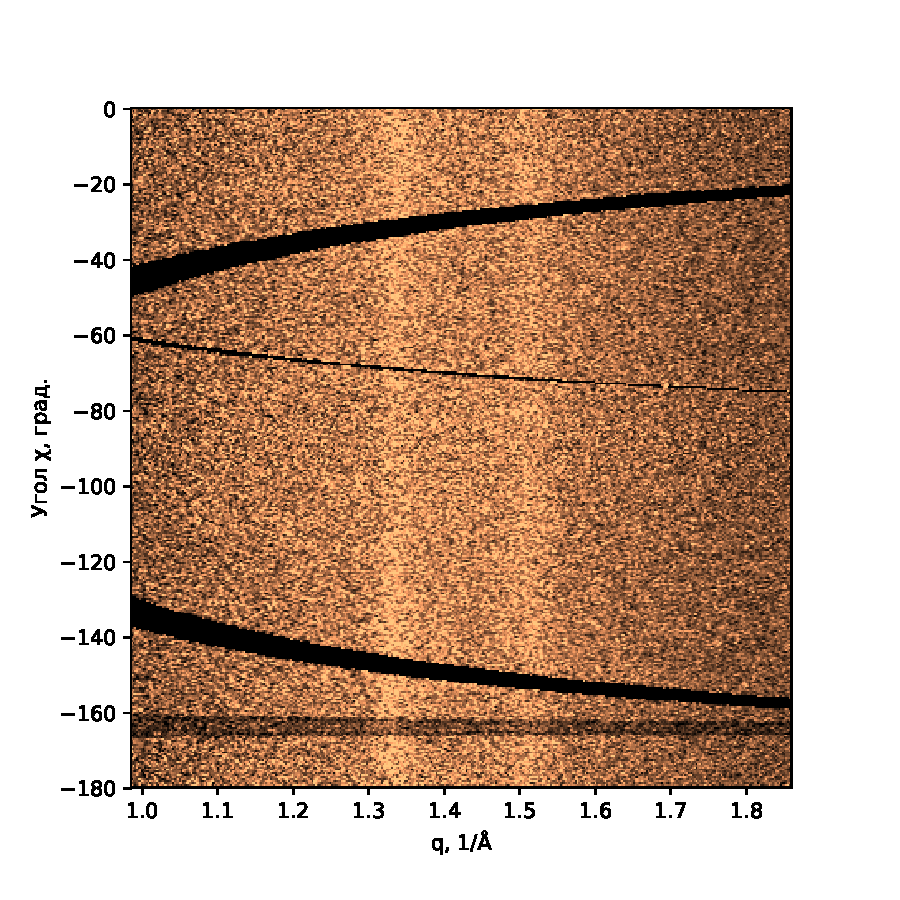
\includegraphics[width=0.5\linewidth]{fig/azim-cryst.pdf}
\end{tabular}
\caption{Фрагменты дифрактограмм (в координатах $(q,\chi)$) в аморфной (слева) и кристаллической (справа) областях.}
\label{fig:azim}
\end{figure}
	
После калибровки, в результате интегрирования по азимутальному углу $\chi$, получаются одномерные профили дифракции. Один из профилей в частично-кристаллической области в широкоугловом диапазоне представлен не рис. \ref{fig:waxs_profile}.

\begin{figure}[h]
    \centering
    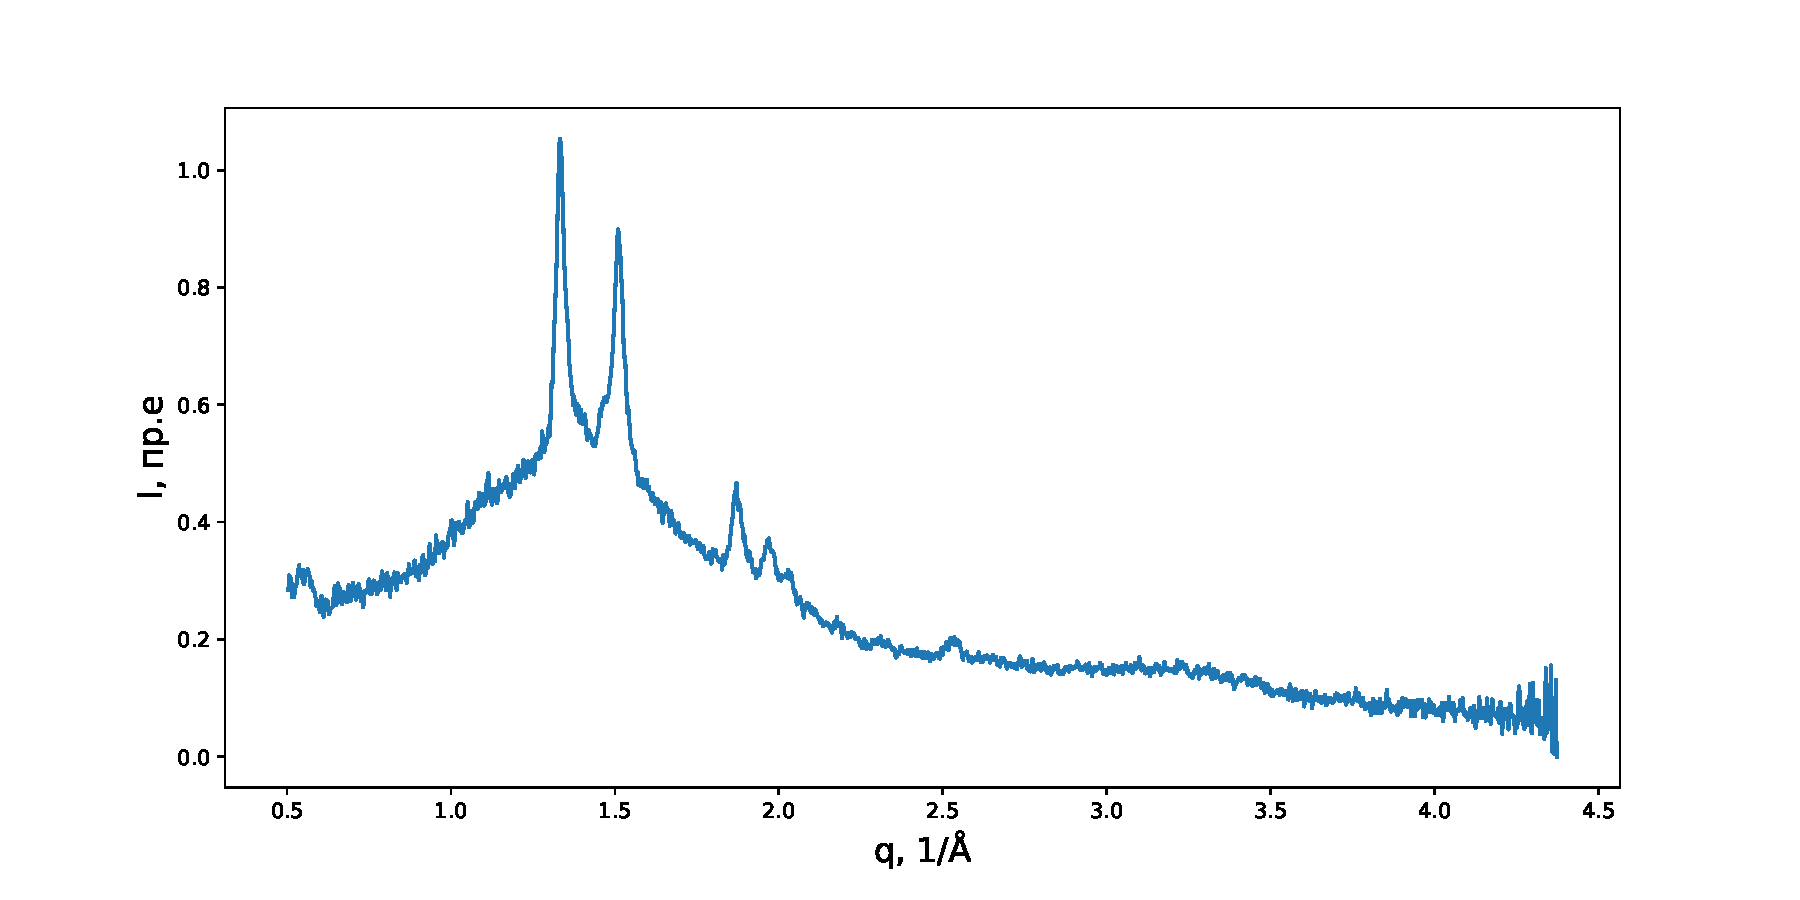
\includegraphics[width=\linewidth]{fig/profile.pdf}
    \caption{Одномерный профиль после азимутального интегрирования}
    \label{fig:waxs_profile}
\end{figure}


	\section{Вычитание фона}
	
	В отличие от обычного фонового шума, широкий сигнал рассеяния от аморфной фазы нельзя определить одним для всех измерений, так как его форма зависит от степени кристалличности. Таким образом, его оценку необходимо проводить для каждого профиля отдельно.
	Стандартные алгоритмы для автоматического распознавания фона, основанные на полиномиальной аппроксимации, показали себя не продуктивными в нашем случае. Распознавание кристаллических пиков и аморфного фона производилось с помощью нелинейного фильтра "rolling ball". В рентгеноструктурном анализе он как правило применяется к двумерным дифрактограммам кристаллических материалов, как например, в работе \cite{ball2018}. Однако подходящая реализация для одномерных профилей, необходимая в случае дифракции на полимерах, не представлена в открытых источниках. Ниже (листинг \ref{lst:ball}) приведена реализация алгоритма для одномерных профилей на языке Python. 
	Идеи для простой реализцации позаимствованы из работы \cite{ball-code}. Ввиду малого отношения сигнал-шум в алгоритме также применяется сглаживание фильтром Савитского-Голея.
\vspace{5px}
	\begin{lstlisting}[language=Python, caption=Алгоритм распознавания фона, label={lst:ball}]
import numpy as np
 
profile = np.load('profile.npy')
r = 40 #ball radius

t1 = np.zeros(profile.shape[0],dtype=np.float32)
for i in range (t1.shape[0]):
    for j in range(-r,r):
        if ((i+j)>0 and (i+j)<t1.shape[0]):
            
            if(t1[i]<profile[i+j]):
                t1[i]=profile[i+j]
                
t2 = np.full(profile.shape[0], 10000,dtype=np.float32)


for i in range (t2.shape[0]):
    for j in range(-r,r):
        if ((i+j)>0 and (i+j)<t2.shape[0]):
            
            if(t2[i]>profile[i+j]):
                t2[i]=profile[i+j]
t3 = np.zeros(profile.shape[0],dtype=np.float32)
count = np.zeros(profile.shape[0],dtype=np.float32)
back = np.zeros(profile.shape[0],dtype=np.float32)

for i in range(t3.shape[0]): #smooth
    for j in range(-r,r):
        if ((i+j)>0 and (i+j)<t3.shape[0]):
            t3[i]+=t2[i+j] #sum
            count[i]+=1
            
    back[i] = t3[i]/count[i] #average
\end{lstlisting}
\vspace{5px}

	Принцип действия алгоритма проиллюстрирован на рис. \ref{fig:ball}. 
	Его можно представить как круг заданного радиуса, который "катится" по профилю.Траектория его центра образует линию, которая и вычитается из начального профиля. Пики, чья ширина меньше радиуса круга, не вычитаются, и остаются в конечном профиле. Так, алгоритм позволяет убирать широкие пика рассеяния аморфной фазы, и оставлять только узкие кристаллические пики.
	
	
	\begin{figure}[ht]
	    \centering
	    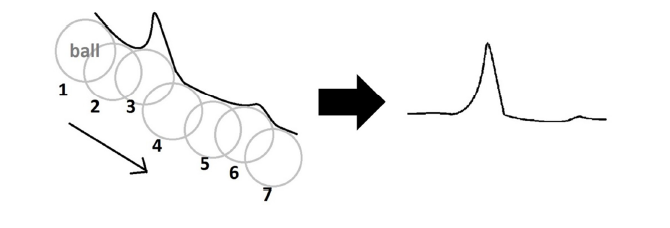
\includegraphics[width=\linewidth]{fig/ball.PNG}
	    \caption{Процедура вычитания фона.}
	    \label{fig:ball}
	\end{figure}

	\section{Аппроксимация пиков}
	
	Как видно из рис. \ref{fig:fitting}, кристаллические пики хорошо аппроксимируются контуром Фойгта, как и полагается пикам рентгеновского рассеяния на кристаллах.
	
		\begin{figure}[ht]\center
\begin{tabular}{rcl}
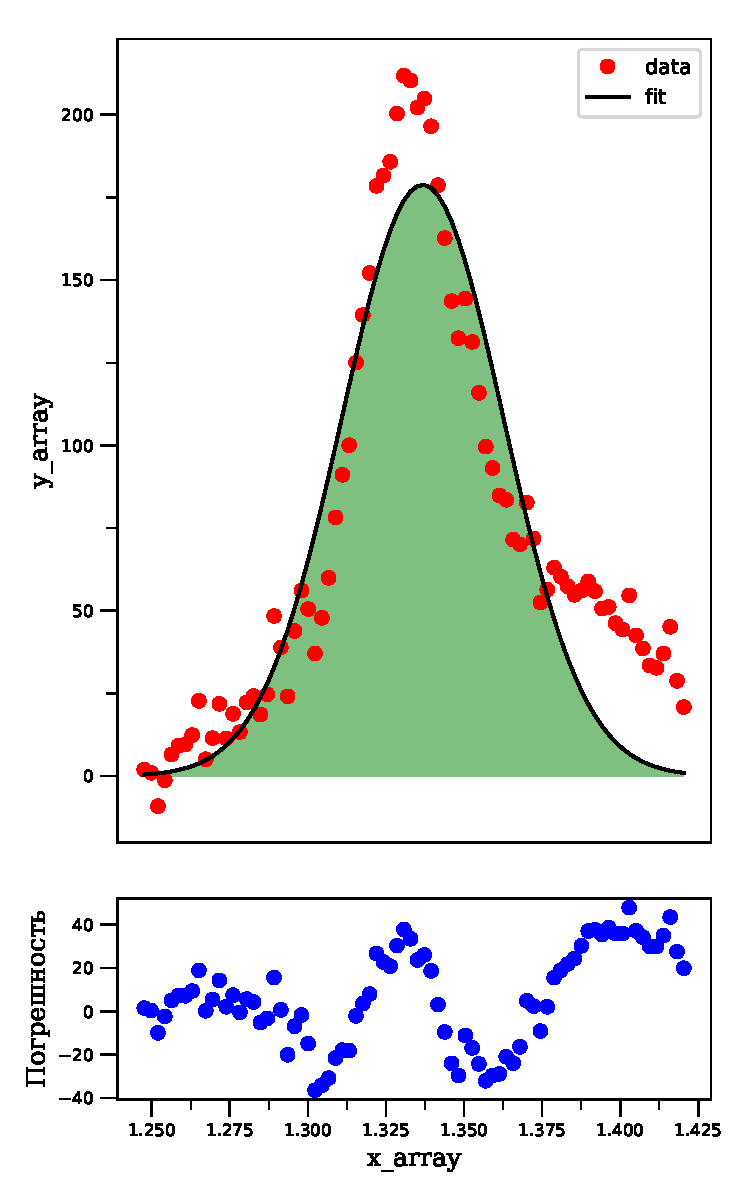
\includegraphics[width=0.33\linewidth]{fig/fitGaussian.pdf}
&
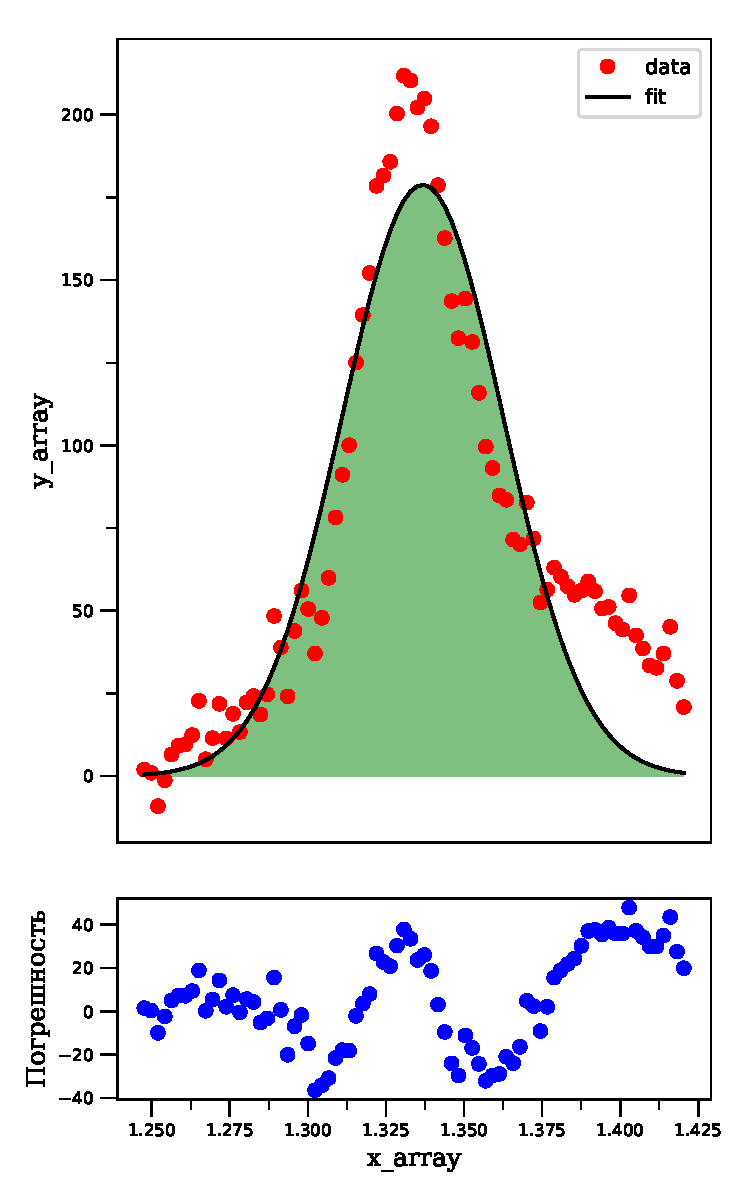
\includegraphics[width=0.33\linewidth]{fig/fitGaussian.pdf}
&
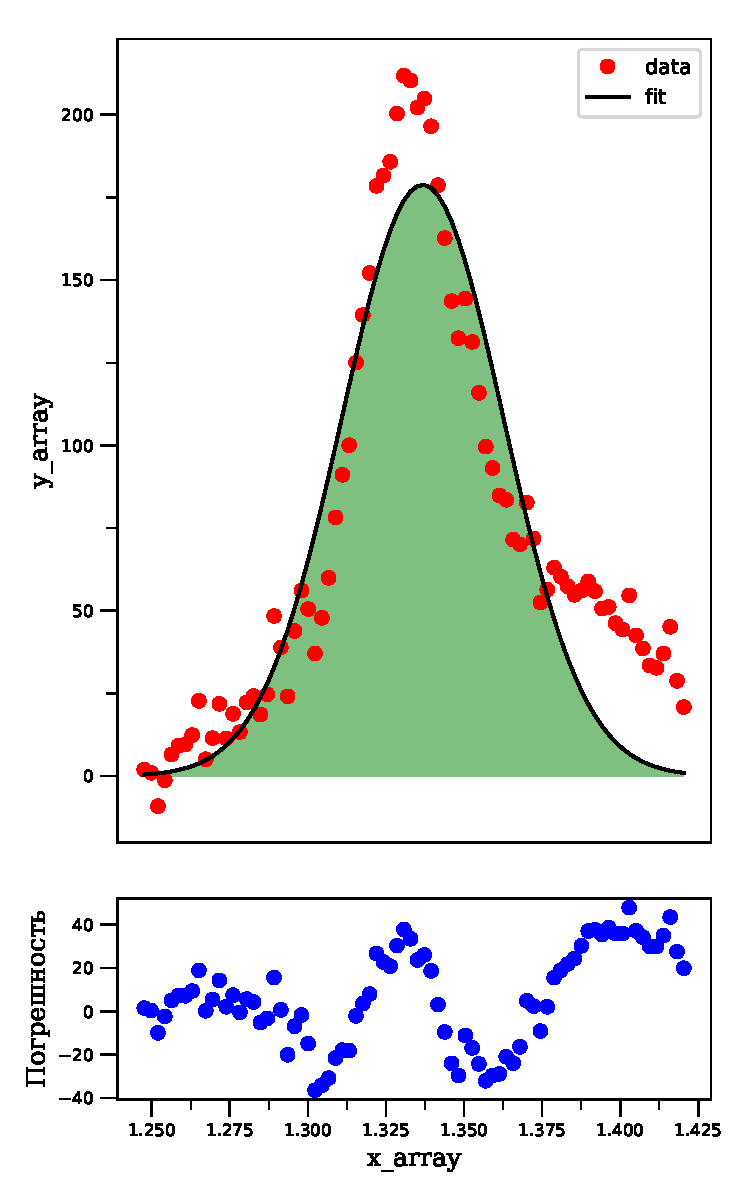
\includegraphics[width=0.33\linewidth]{fig/fitGaussian.pdf}
\end{tabular}
\caption{Фиттинг}
\label{fig:fitting}
\end{figure}
	

	

	\section{Картография образцов}
	\paragraph{Нормализация.}
	
	\paragraph{Частицы порошков.}Составление карт кристалличности образцов показывает, что сами порошки состоят из частичнокристаллических частиц заявленных размеров.
	
	\begin{figure}[h]
	    \centering
	    \begin{tabular}{ccc}
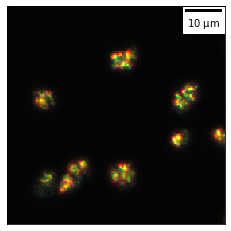
\includegraphics[width=0.33\linewidth]{fig/powder_optic.png}
&
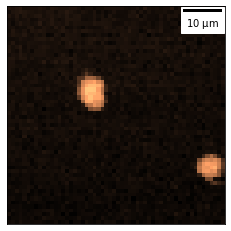
\includegraphics[width=0.33\linewidth]{fig/powder_dif1.png}
&
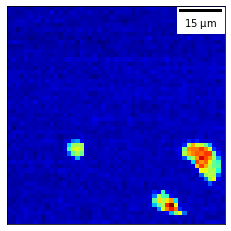
\includegraphics[width=0.33\linewidth]{fig/powder_dif2.png}
\end{tabular}
	    \caption{Отдельные частицы}
	    \label{fig:powder}
	\end{figure}
	
	\paragraph{Область SAXS.}
	Если проинтегрировать область малоуглового рассеяния, можно получить представление о морфологии частиц.
	
	\paragraph{Интенсивность в области WAXS.}
	
	
	
		\begin{figure}[ht]\centering
\begin{tabular}{cc}
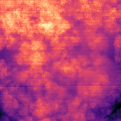
\includegraphics[width=0.5\linewidth]{fig/map-1.png}
&
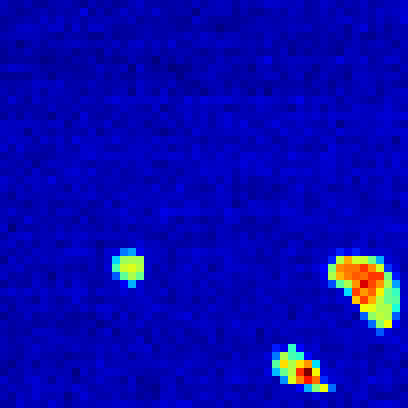
\includegraphics[width=0.5\linewidth]{fig/map-2.png} \\
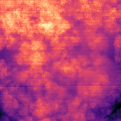
\includegraphics[width=0.5\linewidth]{fig/map-1.png}
&
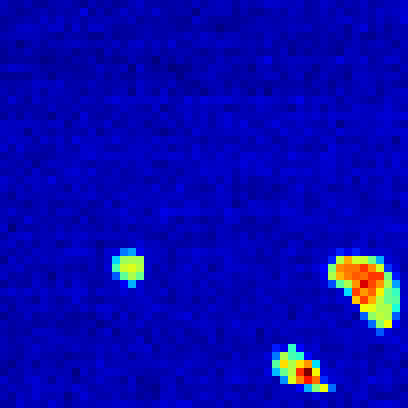
\includegraphics[width=0.5\linewidth]{fig/map-2.png}
\end{tabular}
\caption{Карты кристалличности}
\end{figure}
	
	
	
	
\section{Расчет характеристик}
